\begin{frame}
\begin{center}
\Huge Extra Slides
\end{center}
\end{frame}
%---------------------

% \subsection{Pollutants and health impacts}
\begin{frame}
\frametitle{Pollutants main precursors}
\centering
    \begin{tikzpicture}[
    roundnode1/.style={circle, draw=green!60, fill=green!5, very thick, minimum size=15mm},
    roundnodeP/.style={circle, draw=red!60, fill=red!5, very thick, minimum size=5mm},
    roundnodeS/.style={circle, draw=blue!60, fill=blue!5, very thick, minimum size=5mm},
    ]
    %Nodes
    \node[roundnode1]   (pmm)         at (2,0) {\pmm};
    \node[roundnodeP]   (pmmBC)       [above=of pmm, xshift=-1cm] {BC};
    \node[roundnodeP]   (pmmOC)       [above=of pmm, xshift=1cm] {OC};
    \node[roundnodeS]   (pmmSO2)      [below=of pmm, xshift=-1cm] {SO$_2$};
    \node[roundnodeS]   (pmmNOx)      [below=of pmm, xshift=1cm] {NO$_x$};
    \node[roundnodeS]   (pmmNH3)      [below=of pmm, yshift=-1cm] {NH$_3$};
    \node[roundnode1]   (oo)         at (7,0) {\oo};
    \node[roundnodeS]   (ooVOC)      [below=of oo, xshift=-1cm] {VOC};
    \node[roundnodeS]   (ooNOx)      [below=of oo, xshift=1cm] {NO$_x$};
    \node[roundnodeS]   (ooCH4)      [below=of oo, yshift=-1cm] {CH$_4$};
    
    %Lines
    \draw [->,red]  (pmmBC) to [out=225,in=150] (pmm);
    \draw [->,red]  (pmmOC) to [out=315,in=30] (pmm);
    \draw [->,blue] (pmmSO2) to [out=100,in=250] (pmm);
    \draw [->,blue] (pmmNOx) to [out=80,in=290] (pmm);
    \draw [->,blue] (pmmNH3) -- (pmm);
    \draw [->,blue] (ooVOC) to [out=100,in=250] (oo);
    \draw [->,blue] (ooNOx) to [out=80,in=290] (oo);
    \draw [->,blue] (ooCH4) -- (oo);

    % Simple brace
    \draw [decorate, decoration = {brace,mirror}] (-0.5,3) --  (-0.5,1.5) node [black,midway,xshift=-0.6cm,rotate = 90] {\small{Primary pollutants}};
    \draw [decorate, decoration = {brace}] (-0.5,-4) --  (-0.5,-1.5) node [black,midway,xshift=-1cm,rotate=90,text width=3cm,align=center] {\small{Precursors of secondary pollution}};
    \end{tikzpicture}
\end{frame}

\begin{frame}{Health impacts (mortality) equations}
\begin{center}
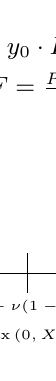
\begin{tikzpicture}[trim left=(concExtra), trim right = (concExtra), node distance = 0.15cm]
    \node (concExtra) at (0,0) {};

    % Equations MORTALITY
    \node (PD1) [below of=concExtra,yshift=0cm,align=center]{\small{$\Delta Mort = y_0 \cdot PAF \cdot pop$}};;
    \node (PAF) [below of=concExtra,yshift=-0.5cm,align=center]{\small{$ PAF = \frac{RR-1}{RR}$}};;

    % timeline    
    \node (LL) [below of=concExtra,xshift=-3cm,yshift=-2.35cm,align=center]{\tiny{$LL(X) = \exp\{\beta(X-X_0)\}$}};;
    \node (IER1) [below of=concExtra,xshift=0cm,yshift=-3.25cm,align=center]{\tiny{$IER(X) = 1-\nu (1-\exp\{-\omega z^\delta\}),$}};;
    \node (IER2) [below of=IER1,align=center,yshift=-0.25cm]{\tiny{$z = \max{(0,X-X_0)}$}};;
    \node (GEMM1) [below of=concExtra,xshift=2.5cm,xshift=1.5cm,yshift=-1.75cm,align=center]{\tiny{$GEMM(X) = \exp\left\{\frac{\theta \log\left(\frac{z}{\alpha+1}\right)}{1+\exp\{-\frac{z-\mu}{\nu}\}}\right\},$}};;
    \node (GEMM2) [below of=GEMM1,align=center,yshift=-0.43cm]{\tiny{$z = X - \min{(X)}$}};;
    
    \node (time) [below of=concExtra,align=center,xshift=5.5cm,yshift=-2.75cm]{\tiny{time}};;
    \draw[->] (-6,-3) -- (6,-3); 
    \draw (-3,-2.75) -- (-3,-3.25);
    \draw (0,-2.75) -- (0,-3.25);
    \draw (4,-2.75) -- (4,-3.25);
\end{tikzpicture}
\end{center}
\end{frame}

\begin{frame}{Health impacts uncertinaty}
\begin{figure}
    \centering
    \includegraphics[width = \linewidth]{extraFigs/heatlh_uncertainty_2030.pdf}
\end{figure}
\vfill \hfill \tiny{\cite{rodes-bachs_beyond_ap}}
\end{frame}

\begin{frame}{Health impacts Kolmogorov-Smirnov test}
\begin{figure}
    \centering
    \includegraphics[width = 0.98\linewidth]{extraFigs/ks_mort_2030_2050.pdf}
\end{figure}
\vfill \hfill \tiny{\cite{rodes-bachs_beyond_ap}}
\end{frame}


% GCAM slides --------------------------------------------------------------------------------------

\begin{frame}{GCAM}
    The Global Change Analysis Model (GCAM) in a figure:
\begin{figure}
    \centering
    \includegraphics[width = 0.5\linewidth]{extraFigs/GCAM_diagram_basic.jpg}
\end{figure}
\vfill\hfill \tiny{Source: \url{https://github.com/JGCRI/gcam-doc}}
\end{frame}

\begin{frame}{GCAM}
\begin{itemize}  \setlength\itemsep{5pt}
    \item The Global Change Analysis Model (GCAM) is an open-source community model developed by Joint Global Change Research Institute (JGCRI) (University of Maryland, MA, USA)
    \item It is a partial-equilibrium, multisector, integrated assessment model designed to explore human and Earth-system dynamics
    \item GCAM analyses the interdependencies between global energy, AFOLU, water, emissions, and climate systems within a single computational platform from now to 2100
    \item The model has been widely used for IPCC scenarios, SSP pathways, and several multisector multiscale studies and reports
\end{itemize}
\end{frame}

\begin{frame}{GCAM evolution}
\begin{figure}
    \centering
    \includegraphics[width = 0.95\linewidth]{extraFigs/GCAM_evolution.jpg}
\end{figure}
\vfill\hfill \tiny{Source: \url{https://github.com/JGCRI/gcam-doc}}
\end{frame}

\begin{frame}{GCAM inputs and outputs}
\begin{figure}
    \centering
    \includegraphics[width = 0.95\linewidth]{extraFigs/GCAM_input_output.png}
\end{figure}
\vfill\hfill \footnotesize{Source: \url{https://github.com/JGCRI/gcam-doc}}
\end{frame}

\begin{frame}{GCAM temporal scale and strucutre}
\begin{figure}
    \centering
    \includegraphics[width = 0.95\linewidth]{extraFigs/GCAM_temporal_structure.jpg}
\end{figure}
\vfill\hfill \tiny{Source: \url{https://github.com/JGCRI/gcam-doc}}
\end{frame}

\begin{frame}{GCAM spatial layers}
    \begin{itemize}
        \item The core version of GCAM divides the entire World in 32 geopolitical regions and 235 water basins
        \item The land regions (384) are the intersection between regions and water basins
        \item There is a single global region for climate system impacts
    \end{itemize}
    \begin{figure}
        \centering
        \includegraphics[width = 0.8\linewidth]{extraFigs/GCAM_spatial_layers.jpg}
    \end{figure}
    \vfill\hfill \tiny{Source: \url{https://github.com/JGCRI/gcam-doc}}
\end{frame}

\begin{frame}{GCAM prices, competition, and funcional forms}
    \begin{columns}[T] 
        \begin{column}{0.48\textwidth} 
            \centering
            \includegraphics[width=\textwidth]{extraFigs/GCAM_prob_approach.png}
        \end{column}
        \begin{column}{0.48\textwidth}
            \begin{itemize} \setlength\itemsep{5pt}
                \item Calibrated logit approach assumes a distribution of realized costs due to heterogeneous conditions
                \item Market share based on probability that a technology has the least cost for an application, avoiding a ``winner take all'' result
                \item Historical calibration influences future competition through the ``share-weight''
            \end{itemize}
        \end{column}
    \end{columns}
    \vfill\hfill \tiny{Source: \url{https://github.com/JGCRI/gcam-doc}}
\end{frame}

\begin{frame}{GCAM ecosystem}
    \begin{figure}
        \centering
        \includegraphics[width = 0.8\linewidth]{extraFigs/GCAM_diagram.jpg}
    \end{figure}
    \vfill\hfill \tiny{Source: \url{https://github.com/JGCRI/gcam-doc}}
\end{frame}
    
% GCAM systems -----------------------------------------------------------------
\begin{frame}{GCAM Energy system}
    \begin{columns}[T] 
        \begin{column}{0.60\textwidth} 
            \centering
            \includegraphics[width=0.6\textwidth]{extraFigs/GCAM_energy_system_breakout.png}
            \includegraphics[width=\textwidth]{extraFigs/GCAM_energy_system.png}
            \vfill\hfill \tiny{Source: \url{https://github.com/JGCRI/gcam-doc}}
        \end{column}
        \begin{column}{0.38\textwidth}
            \begin{itemize}
                \item Regional Energy production, transformation, and end-use demand are based on economic functions of resources, technologies, prices, population, and income
                \item Energy transformation and end-use consumption are represented by specific, bottom-up technologies in most sectors
            \end{itemize}
        \end{column}
    \end{columns}
\end{frame}

\begin{frame}{GCAM Land system}
    \begin{columns}[T] 
        \begin{column}{0.54\textwidth} 
            \centering
            \includegraphics[width=0.6\textwidth]{extraFigs/GCAM_land_system_breakout.png}
            \includegraphics[width=\textwidth]{extraFigs/GCAM_land_system.png}
            \vfill\hfill \tiny{Source: \url{https://github.com/JGCRI/gcam-doc}}
        \end{column}
        \begin{column}{0.45\textwidth}
            \begin{itemize}
                \item All land cover and use, including all commercial land uses as well as non-commercial natural lands, are represented in GCAM
                \item These land categories are represented in each of the 384 land regions (where applicable) and calibrated to match a historical base year
                \item Economics drive future changes in cropland, pasture, forest, and other land uses
            \end{itemize}
        \end{column}
    \end{columns}
\end{frame}
    
\begin{frame}{GCAM Water system}
    \begin{columns}[T] 
        \begin{column}{0.60\textwidth} 
            \centering             
            \includegraphics[width=0.6\textwidth]{extraFigs/GCAM_water_system_breakout.png}
            \includegraphics[width=0.85\textwidth]{extraFigs/GCAM_water_system.png}
            \vfill\hfill \tiny{Source: \url{https://github.com/JGCRI/gcam-doc}}
        \end{column}
        \begin{column}{0.38\textwidth}
            \begin{itemize}
                \item Runoff from Xanthos model with global climate data 
                \item Non-renewable groundwater/depletable resource curves 
                \item Water supply and demand are economically-balanced in each river basin
            \end{itemize}
        \end{column}
    \end{columns}
\end{frame}
    
\begin{frame}{GCAM Climate system}
    \begin{columns}[T] 
        \begin{column}{0.51\textwidth} 
            \centering     
            \includegraphics[width=0.6\textwidth]{extraFigs/GCAM_climate_system_breakout.png}
            \includegraphics[width=\textwidth]{extraFigs/GCAM_climate_system.png}
            \vfill\hfill \tiny{Source: \url{https://github.com/JGCRI/gcam-doc}}
        \end{column}
        \begin{column}{0.48\textwidth}
            \begin{itemize}
                \item GCAM passes emissions to Hector:
                \begin{multicols}{2}
                    \begin{itemize}
                        \item Fossil $CO_2$ (FA)
                        \item Land-Use $CO_2$ (FLC)
                        \item $CH_4$
                        \item $N_2O$
                        \item 26 halocarbons
                        \item Pollutants: $SO_2$, $CO$, $NO_x$, $NMVOC$s, $BC$, $OC$                    
                    \end{itemize}
                \end{multicols}
                \item Hector computes atmospheric $CO_2$ concentrations, radiative forcing (direct and indirect), temperature change, air- land/sea fluxes, ocean heat flux
            \end{itemize}
        \end{column}
    \end{columns}
\end{frame}
    